% Options for packages loaded elsewhere
\PassOptionsToPackage{unicode}{hyperref}
\PassOptionsToPackage{hyphens}{url}
%
\documentclass[
]{article}
\title{Informe HDT1}
\author{Marco Ramirez}
\date{28/1/2022}

\usepackage{amsmath,amssymb}
\usepackage{lmodern}
\usepackage{iftex}
\ifPDFTeX
  \usepackage[T1]{fontenc}
  \usepackage[utf8]{inputenc}
  \usepackage{textcomp} % provide euro and other symbols
\else % if luatex or xetex
  \usepackage{unicode-math}
  \defaultfontfeatures{Scale=MatchLowercase}
  \defaultfontfeatures[\rmfamily]{Ligatures=TeX,Scale=1}
\fi
% Use upquote if available, for straight quotes in verbatim environments
\IfFileExists{upquote.sty}{\usepackage{upquote}}{}
\IfFileExists{microtype.sty}{% use microtype if available
  \usepackage[]{microtype}
  \UseMicrotypeSet[protrusion]{basicmath} % disable protrusion for tt fonts
}{}
\makeatletter
\@ifundefined{KOMAClassName}{% if non-KOMA class
  \IfFileExists{parskip.sty}{%
    \usepackage{parskip}
  }{% else
    \setlength{\parindent}{0pt}
    \setlength{\parskip}{6pt plus 2pt minus 1pt}}
}{% if KOMA class
  \KOMAoptions{parskip=half}}
\makeatother
\usepackage{xcolor}
\IfFileExists{xurl.sty}{\usepackage{xurl}}{} % add URL line breaks if available
\IfFileExists{bookmark.sty}{\usepackage{bookmark}}{\usepackage{hyperref}}
\hypersetup{
  pdftitle={Informe HDT1},
  pdfauthor={Marco Ramirez},
  hidelinks,
  pdfcreator={LaTeX via pandoc}}
\urlstyle{same} % disable monospaced font for URLs
\usepackage[margin=1in]{geometry}
\usepackage{color}
\usepackage{fancyvrb}
\newcommand{\VerbBar}{|}
\newcommand{\VERB}{\Verb[commandchars=\\\{\}]}
\DefineVerbatimEnvironment{Highlighting}{Verbatim}{commandchars=\\\{\}}
% Add ',fontsize=\small' for more characters per line
\usepackage{framed}
\definecolor{shadecolor}{RGB}{248,248,248}
\newenvironment{Shaded}{\begin{snugshade}}{\end{snugshade}}
\newcommand{\AlertTok}[1]{\textcolor[rgb]{0.94,0.16,0.16}{#1}}
\newcommand{\AnnotationTok}[1]{\textcolor[rgb]{0.56,0.35,0.01}{\textbf{\textit{#1}}}}
\newcommand{\AttributeTok}[1]{\textcolor[rgb]{0.77,0.63,0.00}{#1}}
\newcommand{\BaseNTok}[1]{\textcolor[rgb]{0.00,0.00,0.81}{#1}}
\newcommand{\BuiltInTok}[1]{#1}
\newcommand{\CharTok}[1]{\textcolor[rgb]{0.31,0.60,0.02}{#1}}
\newcommand{\CommentTok}[1]{\textcolor[rgb]{0.56,0.35,0.01}{\textit{#1}}}
\newcommand{\CommentVarTok}[1]{\textcolor[rgb]{0.56,0.35,0.01}{\textbf{\textit{#1}}}}
\newcommand{\ConstantTok}[1]{\textcolor[rgb]{0.00,0.00,0.00}{#1}}
\newcommand{\ControlFlowTok}[1]{\textcolor[rgb]{0.13,0.29,0.53}{\textbf{#1}}}
\newcommand{\DataTypeTok}[1]{\textcolor[rgb]{0.13,0.29,0.53}{#1}}
\newcommand{\DecValTok}[1]{\textcolor[rgb]{0.00,0.00,0.81}{#1}}
\newcommand{\DocumentationTok}[1]{\textcolor[rgb]{0.56,0.35,0.01}{\textbf{\textit{#1}}}}
\newcommand{\ErrorTok}[1]{\textcolor[rgb]{0.64,0.00,0.00}{\textbf{#1}}}
\newcommand{\ExtensionTok}[1]{#1}
\newcommand{\FloatTok}[1]{\textcolor[rgb]{0.00,0.00,0.81}{#1}}
\newcommand{\FunctionTok}[1]{\textcolor[rgb]{0.00,0.00,0.00}{#1}}
\newcommand{\ImportTok}[1]{#1}
\newcommand{\InformationTok}[1]{\textcolor[rgb]{0.56,0.35,0.01}{\textbf{\textit{#1}}}}
\newcommand{\KeywordTok}[1]{\textcolor[rgb]{0.13,0.29,0.53}{\textbf{#1}}}
\newcommand{\NormalTok}[1]{#1}
\newcommand{\OperatorTok}[1]{\textcolor[rgb]{0.81,0.36,0.00}{\textbf{#1}}}
\newcommand{\OtherTok}[1]{\textcolor[rgb]{0.56,0.35,0.01}{#1}}
\newcommand{\PreprocessorTok}[1]{\textcolor[rgb]{0.56,0.35,0.01}{\textit{#1}}}
\newcommand{\RegionMarkerTok}[1]{#1}
\newcommand{\SpecialCharTok}[1]{\textcolor[rgb]{0.00,0.00,0.00}{#1}}
\newcommand{\SpecialStringTok}[1]{\textcolor[rgb]{0.31,0.60,0.02}{#1}}
\newcommand{\StringTok}[1]{\textcolor[rgb]{0.31,0.60,0.02}{#1}}
\newcommand{\VariableTok}[1]{\textcolor[rgb]{0.00,0.00,0.00}{#1}}
\newcommand{\VerbatimStringTok}[1]{\textcolor[rgb]{0.31,0.60,0.02}{#1}}
\newcommand{\WarningTok}[1]{\textcolor[rgb]{0.56,0.35,0.01}{\textbf{\textit{#1}}}}
\usepackage{graphicx}
\makeatletter
\def\maxwidth{\ifdim\Gin@nat@width>\linewidth\linewidth\else\Gin@nat@width\fi}
\def\maxheight{\ifdim\Gin@nat@height>\textheight\textheight\else\Gin@nat@height\fi}
\makeatother
% Scale images if necessary, so that they will not overflow the page
% margins by default, and it is still possible to overwrite the defaults
% using explicit options in \includegraphics[width, height, ...]{}
\setkeys{Gin}{width=\maxwidth,height=\maxheight,keepaspectratio}
% Set default figure placement to htbp
\makeatletter
\def\fps@figure{htbp}
\makeatother
\setlength{\emergencystretch}{3em} % prevent overfull lines
\providecommand{\tightlist}{%
  \setlength{\itemsep}{0pt}\setlength{\parskip}{0pt}}
\setcounter{secnumdepth}{-\maxdimen} % remove section numbering
\ifLuaTeX
  \usepackage{selnolig}  % disable illegal ligatures
\fi

\begin{document}
\maketitle

\hypertarget{hoja-de-trabajo-1-analisis-exploratorio}{%
\section{Hoja de Trabajo 1: Analisis
exploratorio}\label{hoja-de-trabajo-1-analisis-exploratorio}}

El objetivo de esta hoja de trabajo era realizar un analisis
exploratorio a la base de datos de peliculas, extraido de IMDB. Es base
cuenta con 10000 filas y con 27 de columnas.

\hypertarget{haga-una-exploraciuxf3n-ruxe1pida-de-sus-datos-para-eso-haga-un-resumen-de-su-conjunto-de-datos.}{%
\subsubsection{1. Haga una exploración rápida de sus datos, para eso
haga un resumen de su conjunto de
datos.}\label{haga-una-exploraciuxf3n-ruxe1pida-de-sus-datos-para-eso-haga-un-resumen-de-su-conjunto-de-datos.}}

\begin{Shaded}
\begin{Highlighting}[]
\FunctionTok{summary}\NormalTok{(datos)}
\end{Highlighting}
\end{Shaded}

\begin{verbatim}
##        id             budget             genres            homePage        
##  Min.   :     5   Min.   :        0   Length:10000       Length:10000      
##  1st Qu.: 12286   1st Qu.:        0   Class :character   Class :character  
##  Median :152558   Median :   500000   Mode  :character   Mode  :character  
##  Mean   :249877   Mean   : 18551632                                        
##  3rd Qu.:452022   3rd Qu.: 20000000                                        
##  Max.   :922260   Max.   :380000000                                        
##  productionCompany  productionCompanyCountry productionCountry 
##  Length:10000       Length:10000             Length:10000      
##  Class :character   Class :character         Class :character  
##  Mode  :character   Mode  :character         Mode  :character  
##                                                                
##                                                                
##                                                                
##     revenue             runtime        video           director        
##  Min.   :0.000e+00   Min.   :  0.0   Mode :logical   Length:10000      
##  1st Qu.:0.000e+00   1st Qu.: 90.0   FALSE:9430      Class :character  
##  Median :1.631e+05   Median :100.0   TRUE :84        Mode  :character  
##  Mean   :5.674e+07   Mean   :100.3   NA's :486                         
##  3rd Qu.:4.480e+07   3rd Qu.:113.0                                     
##  Max.   :2.847e+09   Max.   :750.0                                     
##     actors          actorsPopularity   actorsCharacter    originalTitle     
##  Length:10000       Length:10000       Length:10000       Length:10000      
##  Class :character   Class :character   Class :character   Class :character  
##  Mode  :character   Mode  :character   Mode  :character   Mode  :character  
##                                                                             
##                                                                             
##                                                                             
##     title           originalLanguage     popularity        releaseDate       
##  Length:10000       Length:10000       Min.   :    4.258   Length:10000      
##  Class :character   Class :character   1st Qu.:   14.578   Class :character  
##  Mode  :character   Mode  :character   Median :   21.906   Mode  :character  
##                                        Mean   :   51.394                     
##                                        3rd Qu.:   40.654                     
##                                        Max.   :11474.647                     
##     voteAvg         voteCount      genresAmount    productionCoAmount
##  Min.   : 1.300   Min.   :    1   Min.   : 0.000   Min.   : 0.000    
##  1st Qu.: 5.900   1st Qu.:  120   1st Qu.: 2.000   1st Qu.: 2.000    
##  Median : 6.500   Median :  415   Median : 3.000   Median : 3.000    
##  Mean   : 6.483   Mean   : 1342   Mean   : 2.596   Mean   : 3.171    
##  3rd Qu.: 7.200   3rd Qu.: 1316   3rd Qu.: 3.000   3rd Qu.: 4.000    
##  Max.   :10.000   Max.   :30788   Max.   :16.000   Max.   :89.000    
##  productionCountriesAmount  actorsAmount    castWomenAmount   
##  Min.   :  0.000           Min.   :     0   Length:10000      
##  1st Qu.:  1.000           1st Qu.:    13   Class :character  
##  Median :  1.000           Median :    21   Mode  :character  
##  Mean   :  1.751           Mean   :  2148                     
##  3rd Qu.:  2.000           3rd Qu.:    36                     
##  Max.   :155.000           Max.   :919590                     
##  castMenAmount     
##  Length:10000      
##  Class :character  
##  Mode  :character  
##                    
##                    
## 
\end{verbatim}

\hypertarget{diga-el-tipo-de-cada-una-de-las-variables-cualitativa-ordinal-o-nominal-cuantitativa-continua-cuantitativa-discreta}{%
\subsubsection{2. Diga el tipo de cada una de las variables (cualitativa
ordinal o nominal, cuantitativa continua, cuantitativa
discreta)}\label{diga-el-tipo-de-cada-una-de-las-variables-cualitativa-ordinal-o-nominal-cuantitativa-continua-cuantitativa-discreta}}

\begin{figure}
\centering
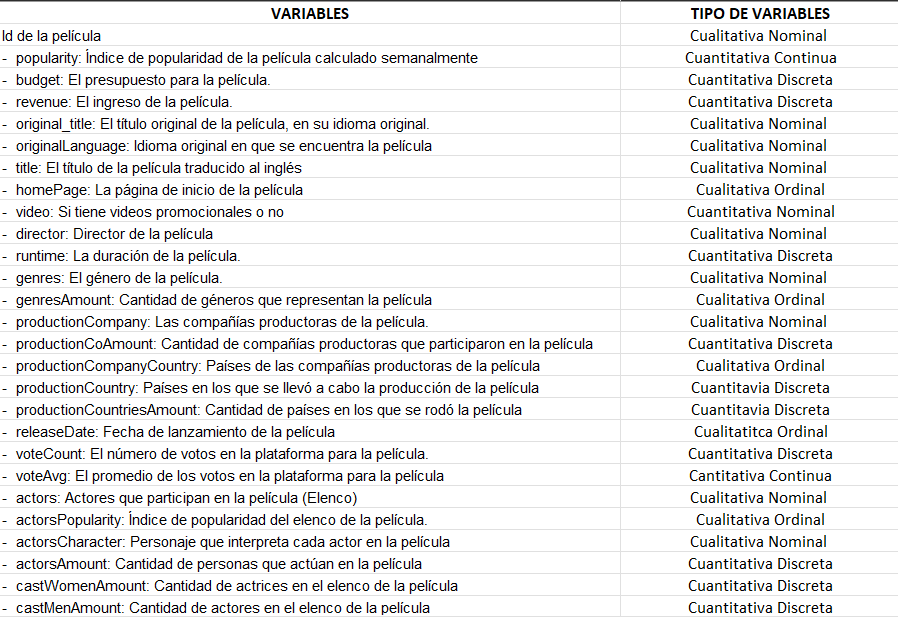
\includegraphics{/Users/MAQUITO/Desktop/UVG/UVG S7/Mineria de datos/HDT1/HDT1_F/HT1_Mineria/Ejercicio2.png}
\caption{Caption for the picture.}
\end{figure}

\hypertarget{responda-las-siguientes-preguntas}{%
\subsubsection{4. Responda las siguientes
preguntas}\label{responda-las-siguientes-preguntas}}

\hypertarget{cuuxe1les-son-las-10-peluxedculas-que-contaron-con-muxe1s-presupuesto}{%
\subsubsection{+ 4.1. ¿Cuáles son las 10 películas que contaron con más
presupuesto?}\label{cuuxe1les-son-las-10-peluxedculas-que-contaron-con-muxe1s-presupuesto}}

Note that the \texttt{echo\ =\ FALSE} parameter was added to the code
chunk to prevent printing of the R code that generated the plot.

\end{document}
